\chapter{Introducción}
% \section{Zona Muerta}
El control clásico es una técnica ampliamente utilizada en ingeniería para el diseño de controladores lineales. Esta metodología ha ganado popularidad debido a las ventajas que brinda, como su simplicidad y la posibilidad de su implementación práctica en una amplia gama de sistemas. Una de las principales fortalezas del control clásico es su enfoque en sistemas lineales, que son relativamente más fáciles de modelar y analizar. Sin embargo, el control clásico todavía enfrenta desafíos importantes, especialmente cuando se trata de lidiar con sistemas no lineales. Estos sistemas presentan características que no pueden ser modeladas o controladas fácilmente mediante técnicas lineales.

El atascamiento y el deslizamiento son fenómenos clave que pueden ocurrir en los sistemas de levitación magnética. El atascamiento se produce cuando el objeto suspendido queda atrapado en una posición determinada y no puede moverse libremente. Por otro lado, el deslizamiento ocurre cuando el objeto no se mantiene estable y se desplaza de manera no deseada.

En este caso particular, el atascamiento-deslizamiento se produce debido a la acción conjunta de dos factores principales: la fricción no lineal y la zona muerta. La fricción no lineal puede provocar deslizamiento cuando la fuerzas de levitación magnética supera a la fuerza de fricción, lo que lleva a movimientos indeseados y una menor estabilidad del sistema. La llamada zona muerta es una de las no linealidades más comunes y desafiantes a las que se enfrenta el control clásico; se refiere a una región en la que no se aplican fuerzas de control al objeto suspendido. Cuando el objeto se encuentra en esta zona muerta, puede quedar atrapado y no responder adecuadamente a las señales de control, lo que resulta en un atascamiento.

Esta zona se refiere a un rango de entrada en el que no se produce ninguna respuesta en la salida del sistema. La presencia de una zona muerta puede ser problemática, ya que afecta la capacidad del controlador para seguir el comportamiento deseado del sistema y puede introducir errores significativos en la respuesta del controlador.

\begin{figure}[!htbp]
  \begin{minipage}[b]{0.4\linewidth}
    \centering
    
\includegraphics[width=\linewidth]{images/zm_fricc/friccion.eps}
    \caption{Fricción no lineal}
    \label{fricción_no_lineal}
  \end{minipage}%
  \hspace{0.2\linewidth} % Aumenta el espacio horizontal
  \begin{minipage}[b]{0.4\linewidth}
    \centering
    
\includegraphics[width=\linewidth]{images/zm_fricc/zm.eps}
    \caption{Zona muerta}
    \label{zona_muerta}
  \end{minipage}
\end{figure}


En los estudios realizados por Diana sobre el fenómeno de atascamiento-deslizamiento, se ha investigado de manera exhaustiva la configuración estable del levitador magnético. El enfoque principal de Diana ha sido comprender los mecanismos detrás del atascamiento y el deslizamiento en esta configuración particular. Para lograrlo, se implementó un sistema de control conmutado que hacía uso de un controlador proporcional integral (PI) y un controlador proporcional derivativo (PD).

En el marco de investigación desarrollado por Arturo, se procedió a realizar un modelo y validar lo que se denomina como "zona muerta dura". Mediante esta validación, fue posible obtener una comprensión más precisa y detallada de los efectos del atascamiento y el deslizamiento en los motores de imanes permanentes. Además, se implementó un controlador con doble efecto integral  que permitió que el motor se mantuviera en la zona muerta dura durante un tiempo reducido, optimizando así su rendimiento general.

La zona muerta inversa se ha propuesto como una solución para abordar el problema de la zona muerta en sistemas de control. La idea detrás de la zona muerta inversa es compensar esta falta de respuesta mediante la aplicación de una señal de control adicional. Esta señal se genera utilizando información sobre la zona muerta y su ubicación precisa. Sin embargo, lograr una delimitación precisa de la zona muerta puede ser un desafío, ya que puede depender de diversos factores, como el diseño del sistema, las características de los sensores y la incertidumbre en las mediciones.


\begin{figure}[htbp]
    \centering
    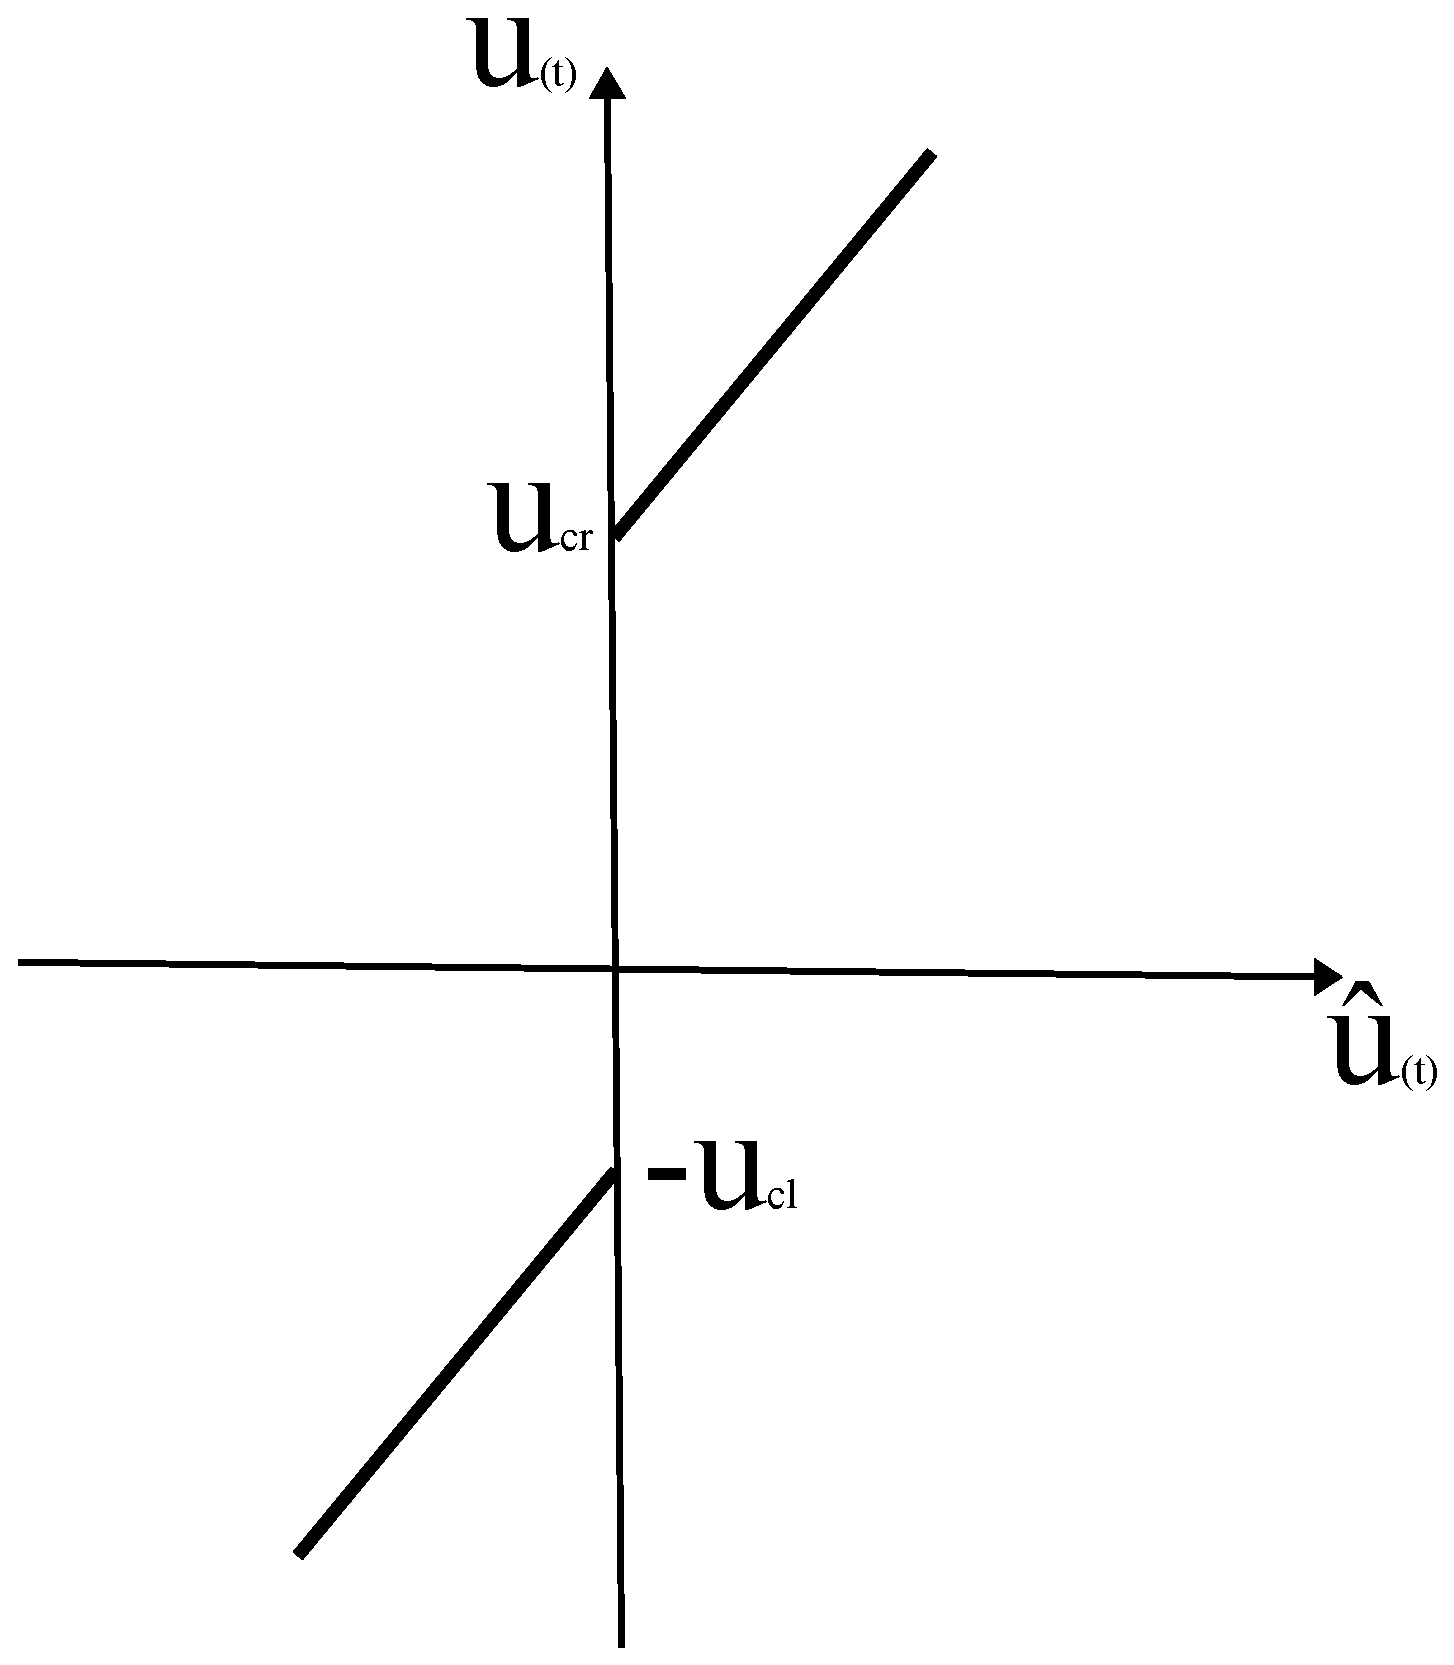
\includegraphics[width=0.3\textwidth]{images/zm_fricc/zm_inversa.eps}
    \caption{Zona muerta inversa}
    \label{zonamuerta}
\end{figure}


Además de la dificultad en la delimitación precisa de la zona muerta, la implementación de la zona muerta inversa ha presentado otro problema: el castañeo o chattering. Este fenómeno se caracteriza por oscilaciones rápidas y no deseadas en la señal de control, lo que puede afectar negativamente el rendimiento y la estabilidad del sistema de control. El castañeo puede ser especialmente problemático en simulaciones, donde los errores numéricos y la discretización de las señales pueden agravar el fenómeno.

Los desafíos encontrados en la implementación de la zona muerta inversa han resultado en una notable falta de investigaciones experimentales en este tema. A pesar de los avances teóricos y las simulaciones realizadas hasta el momento, es evidente la escasez de artículos que se enfoquen en su desarrollo a través de experimentos de laboratorio. Esta carencia puede ser atribuida a la complejidad y las dificultades prácticas asociadas con la implementación de esta técnica en entornos reales. No obstante, esta falta de evidencia no nos permite concluir que la zona muerta inversa no sea una solución efectiva para el problema en cuestión.

La investigación está encaminada a el estudio del modelo del Sistema de Levitación Magnética en su configuración inestable, basándose en el artículo y tesis de Diana en el cual se hizo uso del método de ajuste de curvas, concretamente mediante un ajuste polinomial, para mejorar la precisión de los parámetros del modelo y obtener resultados más fiables en relación con los datos experimentales. Esto permite trabajar sobre un modelo validado.

El campo de acción abordado en este estudio se encuentra enmarcado en la aplicación de la simulación como una herramienta que posibilita un exhaustivo análisis de las propiedades y características del SLM en un entorno virtual controlado. A través del empleo de Matlab, se simulan las condiciones y variables necesarias para representar fielmente el comportamiento del sistema.
La simulación en sí misma permite recrear situaciones y escenarios que podrían ser difíciles de obtener en la realidad, además de ofrecer la capacidad de modificar y ajustar parámetros específicos para examinar su influencia en el desempeño del SLM. De esta manera, se logra una comprensión más profunda de la dinámica del sistema en su configuración inestable.


% \subsection{Modelos matemáticos de la fuerza electromagnética}
Fue llevado a cabo una extensa revisión de la bibliografía existente sobre los diferentes modelos de levitación magnética. Se analizaron diversos estudios y publicaciones científicas que abordaban este tema, encontrándose una gran cantidad de modelos equivalentes entre sí. La diferencia de estos modelos está en su representación de la fuerza electromagnética.

Con el fin de mejorar la coherencia del modelo matemático completo del sistema y facilitar su simulación, se realiza la transformación de las ecuaciones al espacio de estados, estableciendo las siguientes equivalencias:


\begin{align*}
    &x_{1}=x \\ \thinspace
    &x_{2}=\dot{x} \\ \thinspace
    &x_{3}=i \\ \thinspace
    &u=v(t) \\ \thinspace
\end{align*} 

considerando que $(x_{1},x_{2},x_{3},u)$ son la posición, velocidad, corriente y voltaje de control, respectivamente.



\begin{enumerate}
    \item {
        \begin{align*}
        &F_{em}=\frac{L_{r}}{2a}i^2e^{-\frac{x}{a}} \\ \thinspace
    \end{align*} 


    Se observa una disminución en la inductancia terminal $L_{r}$ de la bobina cuando el objeto a levitar se encuentra cerca de $x=0$. La inductancia está influenciada por la posición $x$ de la bobina sobre el objeto  y presenta una decaída que sigue una escala de longitud $a$, la cual varía en función del tamaño del objeto y las dimensiones de la bobina.
            
            }
    
    \item {
        \begin{align*}
        &F_{em}=K_{1}\left(\frac{x_{3}}{x_{1}}\right)^2 \\ \thinspace
    \end{align*} 

    En esta ecuación, la fuerza electromagnética se comporta de manera lineal decreciente cuando se tienen valores negativos de la ganancia $K_{1}$. Sin embargo, la posición real nunca puede ser cero, ya que la esfera siempre se encontrará en una posición deseada distinta de cero. Desde el punto de vista matemático, la fuerza electromagnética podría ser infinita, lo cual generaría un problema en la simulación numérica. 

            }

    \item {
        \begin{align*}
        &F_{em_{u}}=\frac{u}{a(x_{1}+b)^N} \\ \thinspace
    \end{align*} 
    
    En la expresión anterior se muestra una aproximación del modelo matemático dinámico, en el cual las constantes a, b y N son determinadas por modelos numéricos o métodos empíricos. Es necesario aproximar la ecuación utilizando parámetros constantes en la región de interés. No obstante, debido a la no linealidad del campo electromagnético, puede haber variaciones en esas constantes cuando la fuerza que puede experimentar el sistema es alta. 
          
          }

    \item {
        \begin{align*}
        &F_{em}=\frac{x_{3}^2}{1,1994x_{1}^4-0,9165x_{1}^3+0,7159x_{1}+0,0304} \\ \thinspace
    \end{align*} 

    Se puede aproximar este modelo mediante un polinomio de cuarto orden, de acuerdo al comportamiento real del levitador que se esté analizando o implementando. En esta aproximación, se consideran la corriente y la posición como factores determinantes.
    
          }

\end{enumerate}






En base a esta revisión, se ha tomado la decisión de adoptar el modelo que ha sido ampliamente estudiado en la práctica, específicamente en el artículo y la tesis de Diana, los cuales han sido referenciados en otros trabajos de investigación y han sido respaldados por experimentos reales.

La realización en espacio de estados para el caso inestable es:

\begin{itemize}[label={}]
    \item{
    
    \begin{align*}
        &F_{em}= \dfrac{u}{bm(h+a-x_{1})^4} 
    \end{align*}
    
    
    Se observa que la fuerza electromagnética se expresa como una función de cuarto grado que depende directamente del voltaje de control  e inversamente de la distancia. Los parámetros $a$ y $b$ son obtenidos experimentalmente, siendo $h$ la altura sobre la cual el disco se desplaza.
    }
    
\end{itemize}

Cabe destacar que esta elección se basa también en las recomendaciones proporcionadas por el fabricante del modelo en cuestión, tal como se menciona en la documentación correspondiente. Además, se ha comprobado que este modelo ha demostrado su funcionamiento satisfactoriamente en diversas ocasiones.

Al recurrir a este modelo específico, se busca aprovechar los avances y conocimientos generados por la comunidad científica en torno a su diseño y rendimiento. Su elección se respalda tanto en la investigación académica como en la experiencia práctica, lo cual brinda una mayor confianza en su efectividad y resultados.

\section{Modelo en configuración inestable}

En el ámbito de la literatura especializada, hasta el momento no se ha abordado de manera exhaustiva un problema que involucra el fenómeno del atascamiento-deslizamiento inestable. Dada esta falta de exploración y comprensión profunda, resulta necesario abordar dicho problema con el fin de ampliar nuestro conocimiento y contribuir al avance científico.

En este sentido, nos proponemos dirigir nuestra atención hacia el sistema del levitador en una configuración específica y particularmente inestable. Cabe destacar que se ha reportado la aparición de este fenómeno en un artículo y una tesis elaborados por Diana, los cuales proporcionan información valiosa sobre el tema.


\begin{figure}[htbp]
    \centering
    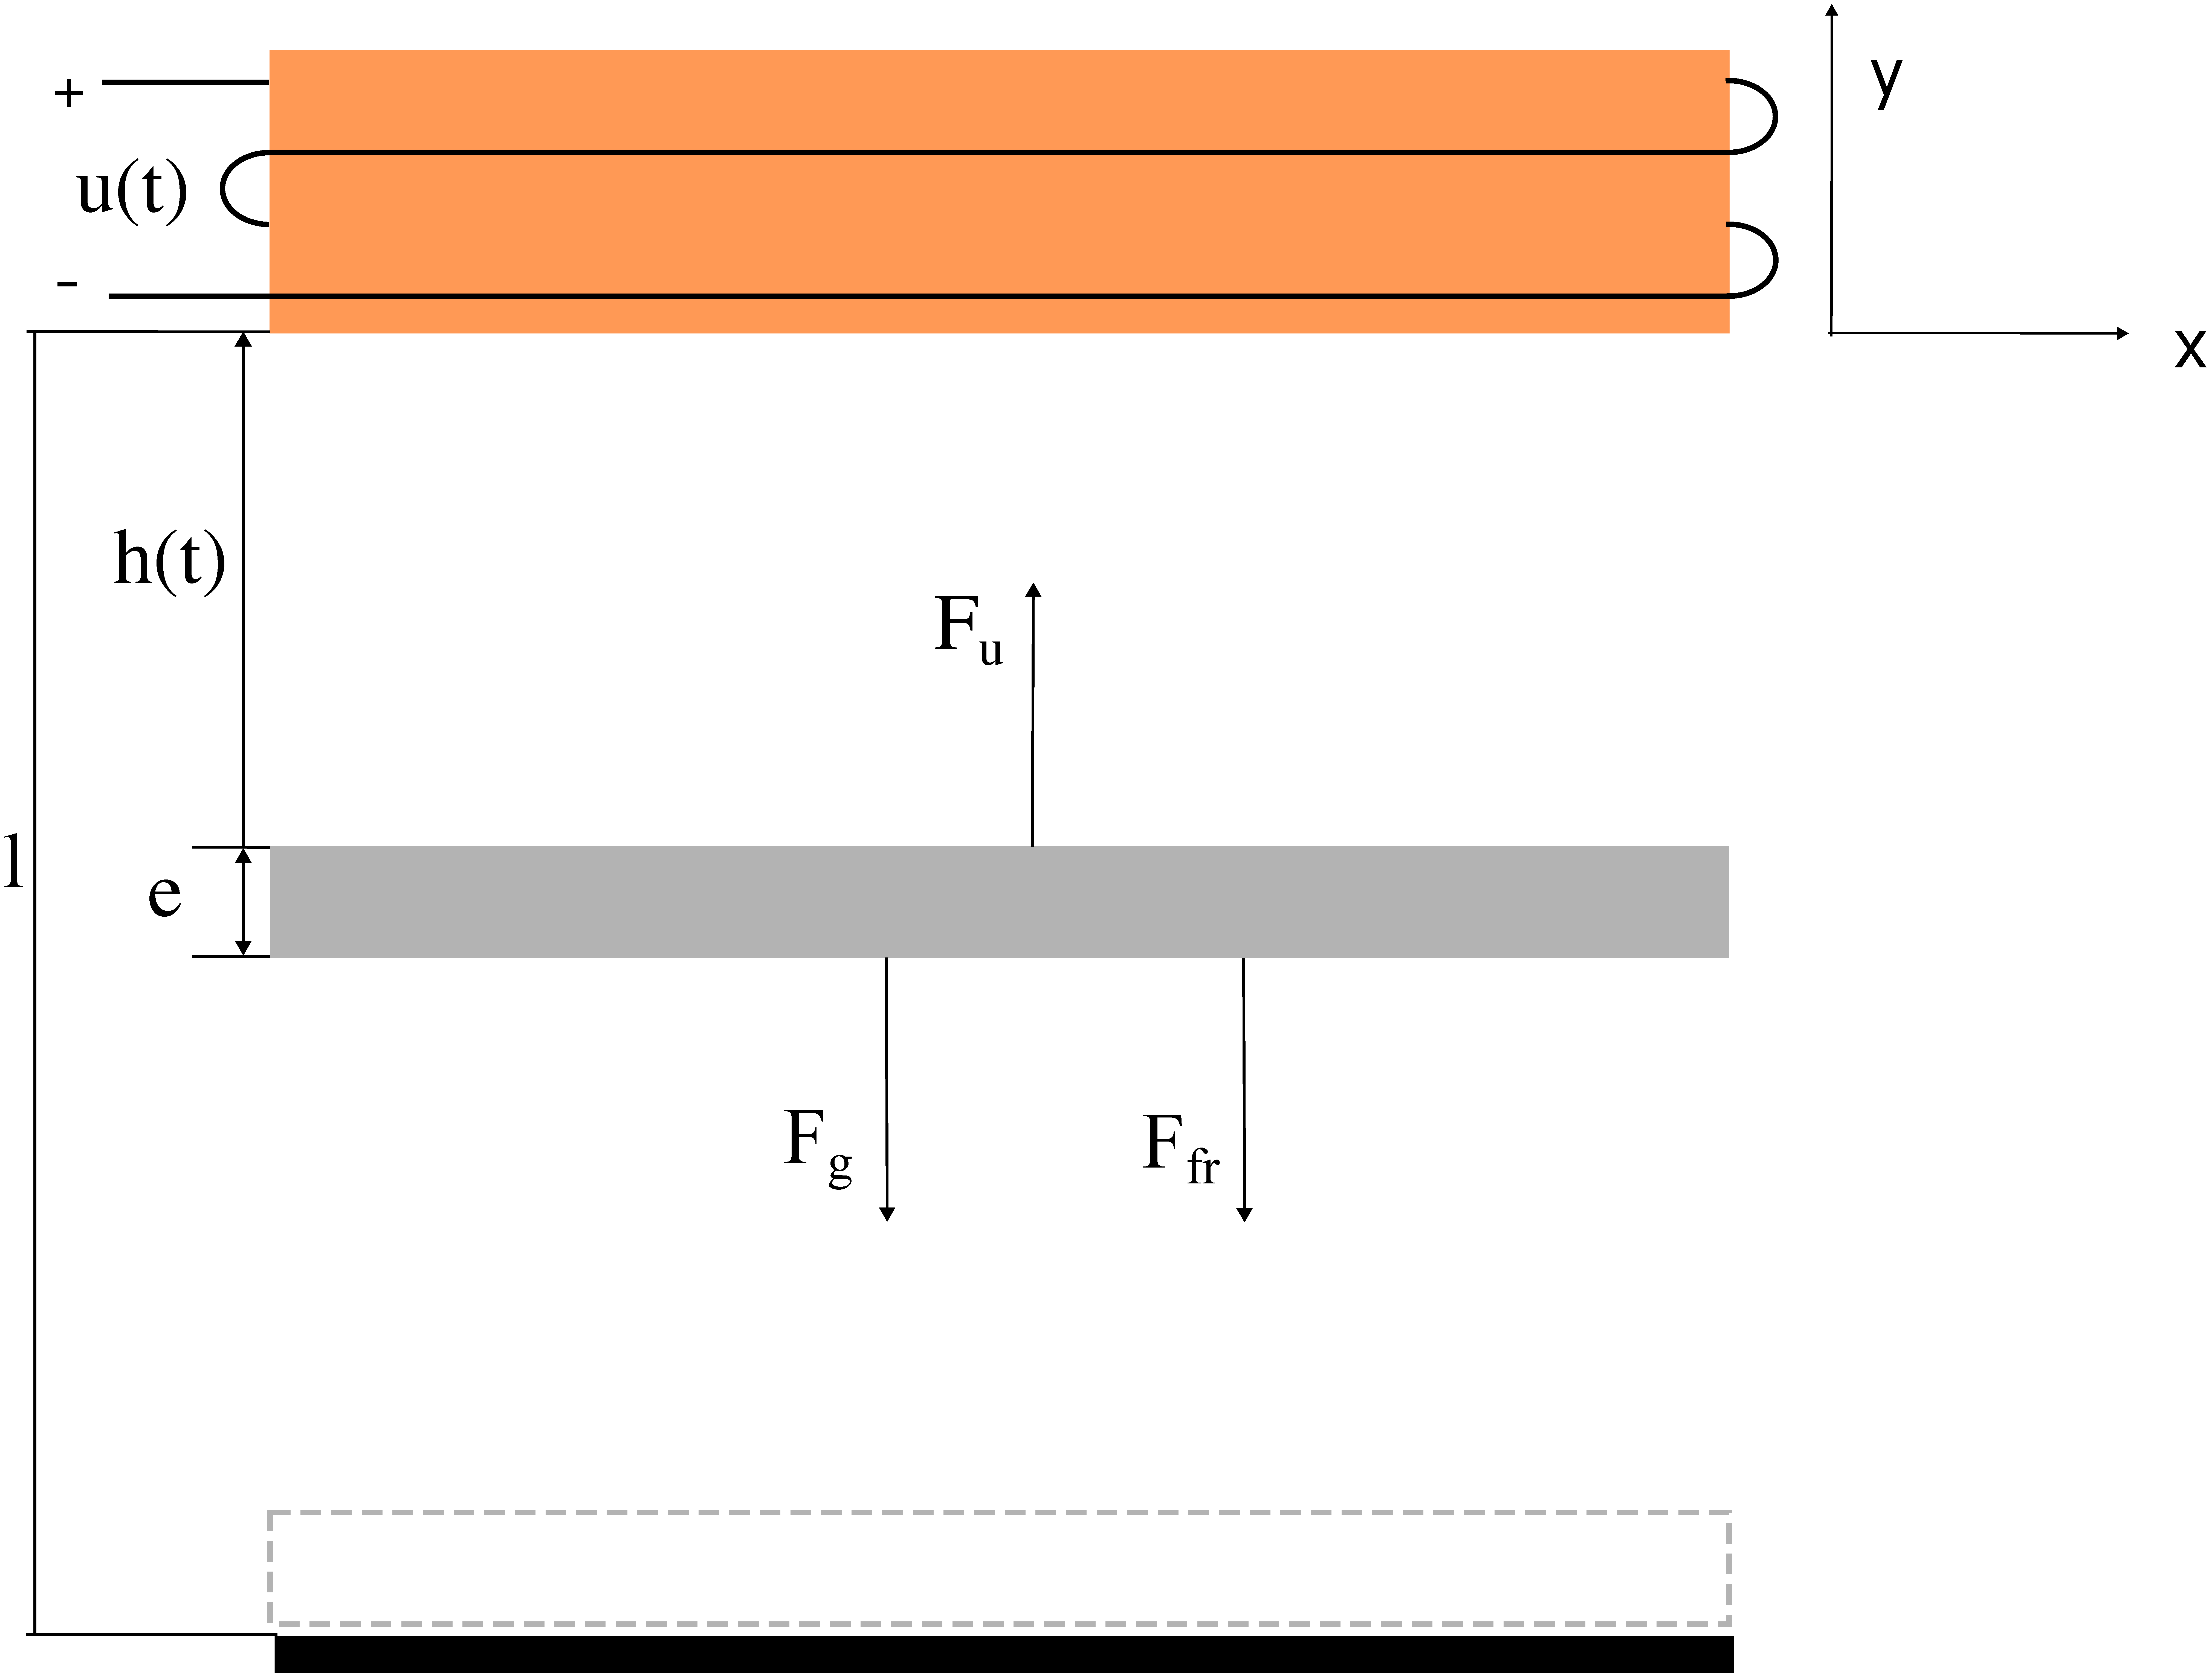
\includegraphics[width=0.5\textwidth]{images/configurations/configuracion_inestable.eps}
    \caption{SLM en configuración inestable}
    \label{SLMinestable}
\end{figure}


Sin embargo, nos enfrentamos a un desafío significativo debido a la indisponibilidad del equipo requerido para llevar a cabo experimentos directos. Afortunadamente, contamos con una alternativa viable para abordar esta limitación: la simulación. Por lo tanto, hemos optado por realizar un estudio exhaustivo y detallado utilizando técnicas de simulación que nos permitirán explorar y comprender los aspectos fundamentales del fenómeno de atascamiento-deslizamiento inestable en el sistema del levitador.

Al emplear esta metodología, buscamos obtener resultados concluyentes y fiables que contribuyan a llenar el vacío existente en la literatura y aporten una perspectiva más amplia sobre este problema particular. Además, esta aproximación nos permitirá evaluar diferentes escenarios y condiciones de manera controlada, brindándonos una mayor comprensión de los factores que influyen en el fenómeno y sus posibles implicaciones prácticas.

Se tuvieron en cuenta como consideraciones iniciales  considerar la fricción lineal. La elección de la zona muerta dura fue seleccionada debido a su capacidad de proporcionar un contraste más sólido con la realidad.

\begin{figure}[htbp]
    \centering
    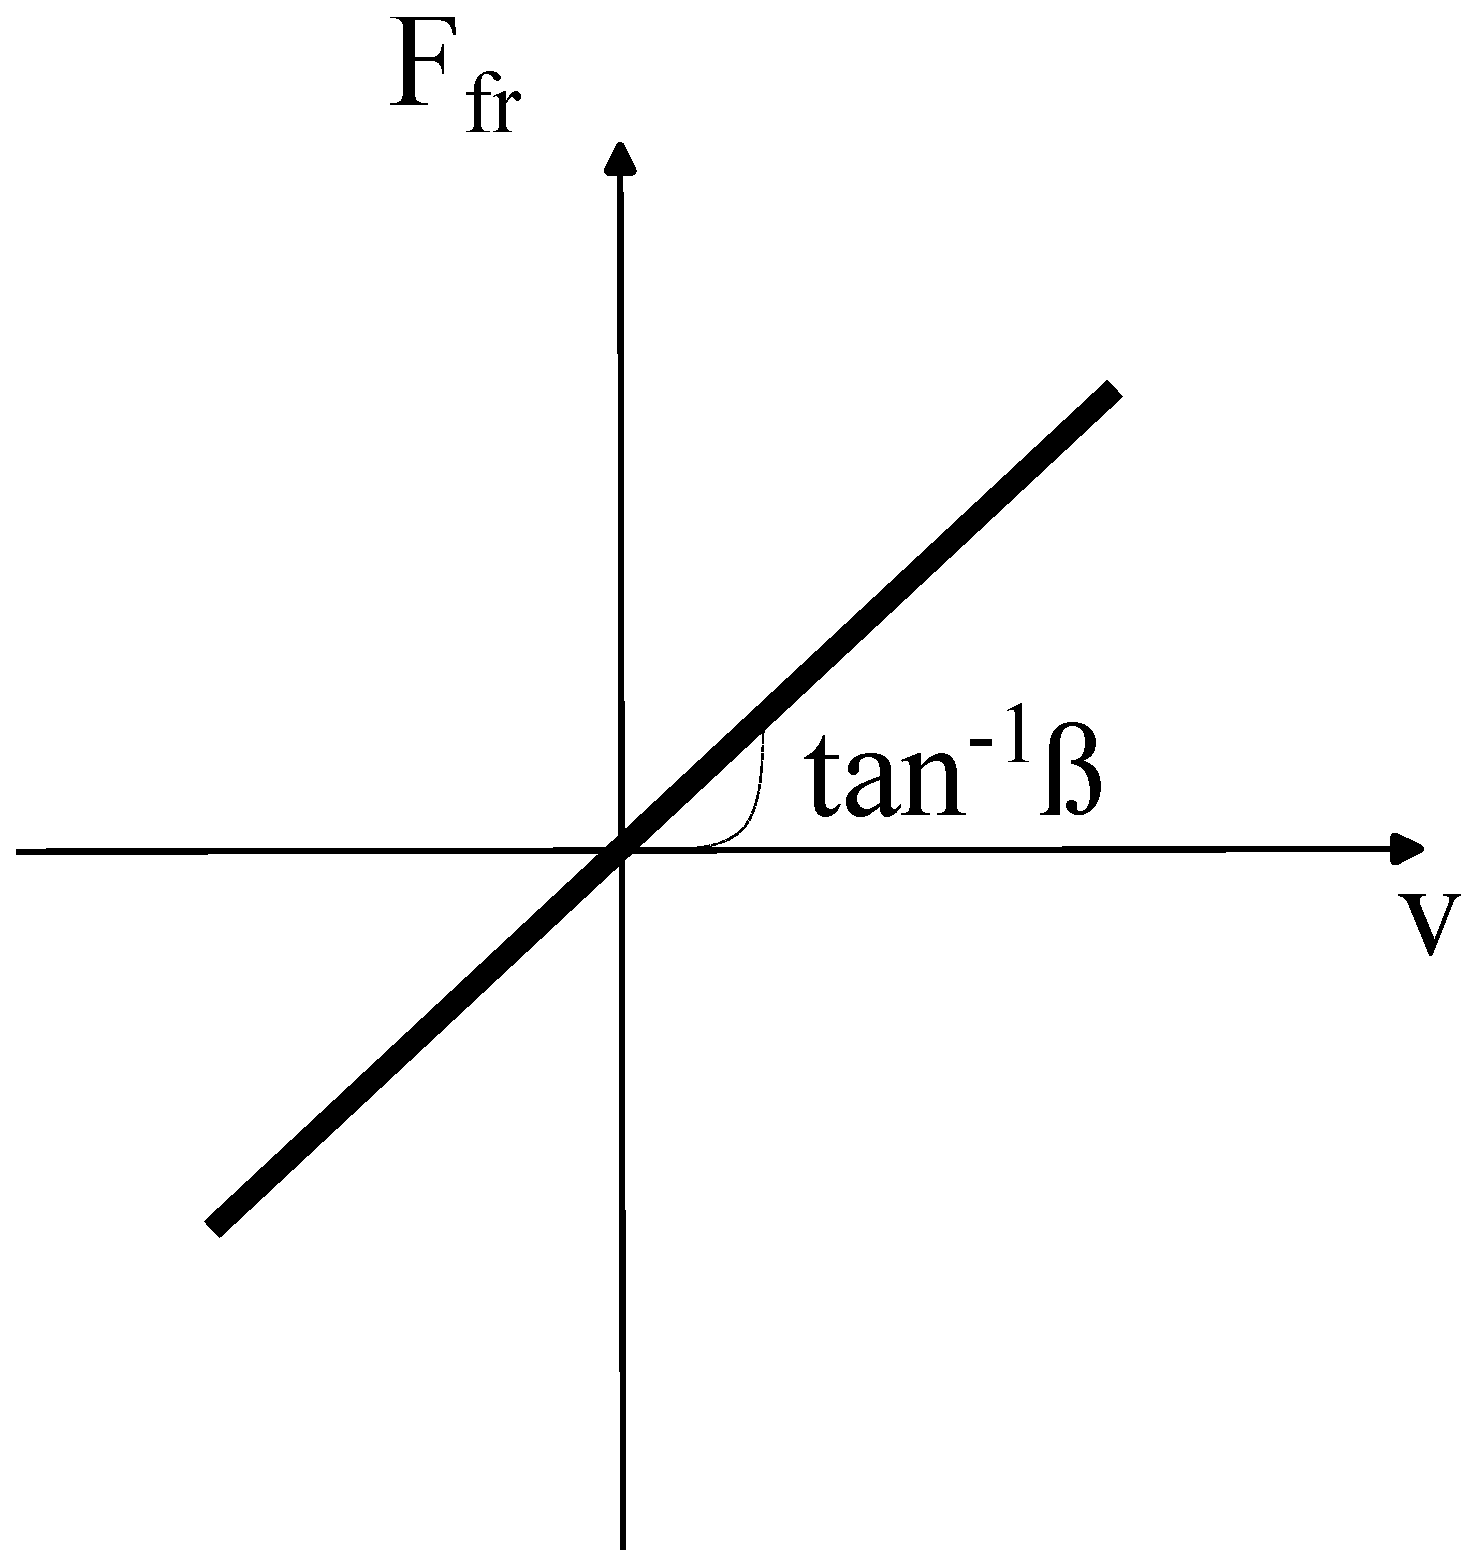
\includegraphics[width=0.3\textwidth]{images/zm_fricc/friccionlineal.eps}
    \caption{Fricción lineal}
    \label{friccionlineal}
\end{figure}

Hay que tener en cuenta que en los levitadores magnéticos tanto su versión estable como la inestable la zona muerta es dinámica y está en función del voltaje y la velocidad de equilibrio.

\begin{figure}[htbp]
  \begin{minipage}[b]{0.35\linewidth}
    \centering
    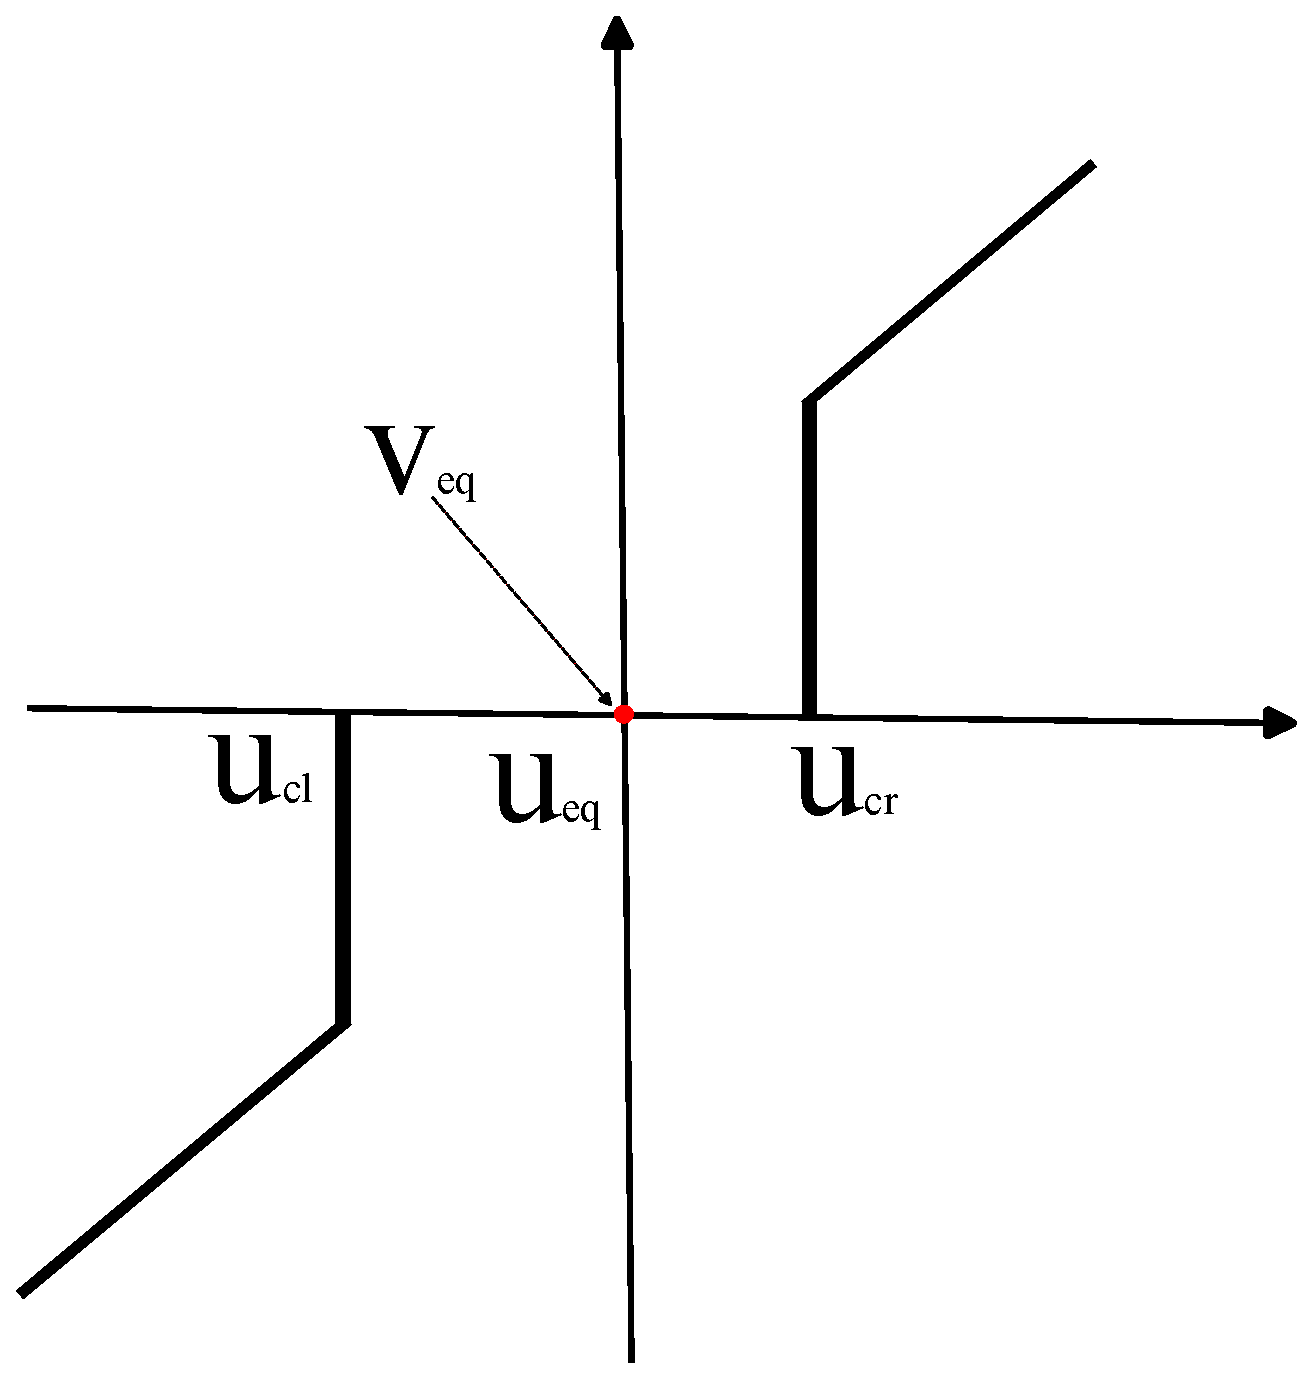
\includegraphics[width=\linewidth]{images/zm_fricc/zm_estatica.eps}
    \caption{Zona muerta estática}
    \label{zmestatica}
  \end{minipage}%
  \hspace{0.2\linewidth} % Aumenta el espacio horizontal
  \begin{minipage}[b]{0.4\linewidth}
    \centering
    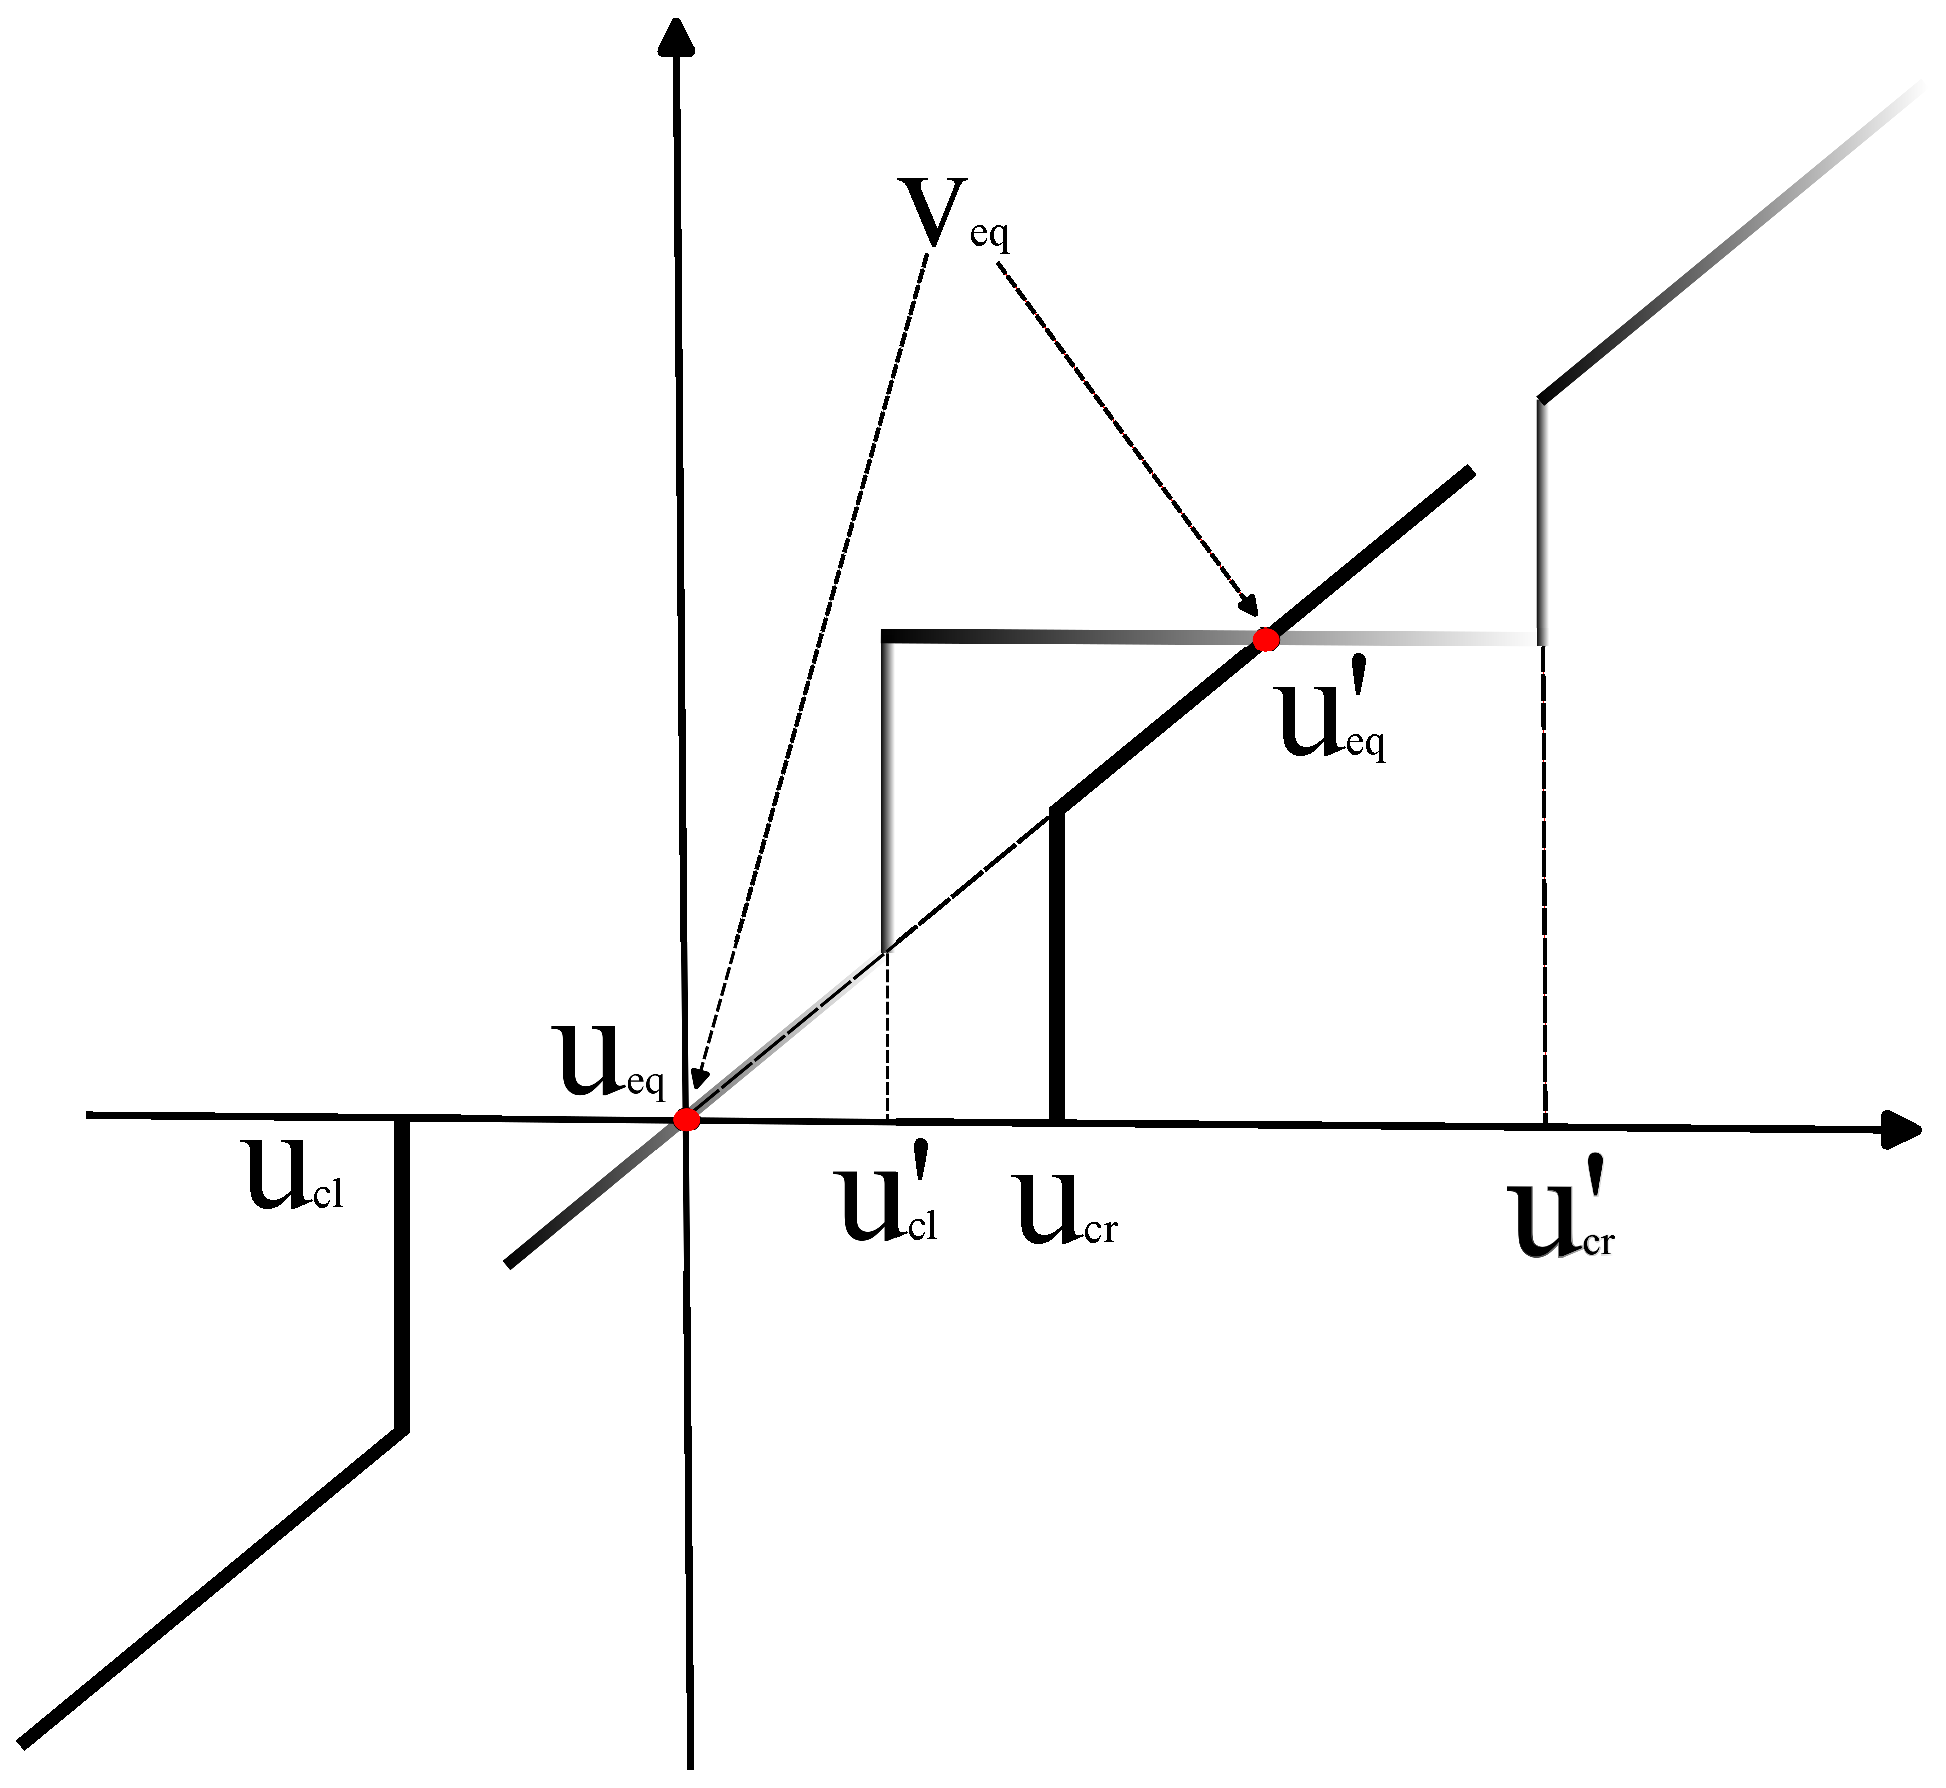
\includegraphics[width=\linewidth]{images/zm_fricc/zm_dinamica.eps}
    \caption{Zona muerta dinámica}
    \label{zmdinamica}
  \end{minipage}
\end{figure}

La ecuación que modela el SLM según el diagrama de fuerzas sobre el cuerpo a levitar es\cite{galuppini}\cite{yeh}\cite{yang}:

\begin{equation}
m\ddot{h}_{(t)}=F_{u}-F_{g} -F_{fr}
\end{equation}

Donde $F_{u}$ es la fuerza del electroimán, $F_{g}$ es la fuerza de gravedad y $F_{fr}$ la fuerza de fricción.

La fuerza magnética puede ser modelada para el caso inestable como:
\begin{equation}
F_{u}=\dfrac{u}{b[a+l+e-h(t)]^4}\
\end{equation}

De (1) y (3), la ecuación no lineal de movimiento resulta para el sistema inestable:
\begin{equation}
\ddot{h}(t)=\dfrac{u}{mb[a+l+e-h(t)]^4}-c_{1}\dot{h}(t)-g
\end{equation}

con $c_{1}=c/m.$\\
Donde $m$ [Kg] es la masa del imán, $h$ [cm] es la distancia entre la bobina y el imán en centímetros, $c$ es el coeficiente de fricción, $g$ es la aceleración debido a la fuerza de gravedad, $a$ y $b$ son constantes, $l$ es la longitud de la barra de vidrio, $e$ es ell espesor del disco del imán y $u$ es el esfuerzo de control en Volts.
\section*{Modelado en espacio de estados}
Si se propone el cambio de variable
\begin{align*} 
&x_{1}=  h(t) \\ 
&\dot{x}_{1}=x_{2}
\end{align*}

La realización en espacio de estados para el caso inestable es:

\begin{align*}
    &\dot{x_{1}}=x_{2}\\
    &\dot{x_{2}}= \dfrac{u}{bm(h+a-x_{1})^4} -c_{1}x_{2} - g
\end{align*}

\section*{Linealización}

Considerando que el sistema se encuentra en un estado equilibrio:

Para el caso inestable
\begin{align*}
    &0=x_{2}\\
    &0=  \dfrac{u}{bm(h+a-x_{1})^4}-c_{1}x_{2} - g
\end{align*}
Se tiene que: 

\begin{align*}
    &x_{1}^{*}={{\left(\dfrac{u}{b\,g\,m}\right)}}^{1/4} -(a+h)\\
    &x^{*}_{2}=0
\end{align*}

Para el caso inestable
\begin{equation}
    \dot{z}=\left(\begin{array}{cc}
0 & 1\\\\
-\dfrac{4}{{{\left(\dfrac{u}{b\,g\,m}\right)}}^{1/4}} & c_{1}
\end{array}\right)z + \left(\begin{array}{c}
0\\\\
\dfrac{1}{b\,m\,{{\left(a+h-x^{*}_1 \right)}}^4 }
\end{array}\right)u
\end{equation}

El polinomio característico del sistema linealizado está dado por:

\begin{equation}
 \lambda^2 -c_{1}\,\lambda+\dfrac{4 }{{{\left(\dfrac{u}{b\,g\,m}\right)}}^{1/4}}=0 
\end{equation}
El polinomio no es Hurwitz en todos los puntos de equilibrio, por lo que los puntos de equilibrio del sistema son asintóticamenta inestables localmente.


\section{Dificultades encontradas}

Se han experimentado varios inconvenientes durante la simulación. En primer lugar, se encontró una incompatibilidad de variables en el entorno de simulación Simulink, lo cual hizo imposible encontrar una solución adecuada. El entorno de integración numérica utilizado en Simulink no permite la integración por lapsos, lo que limitó aún más las posibilidades de encontrar una solución viable.

Con el objetivo de superar estas dificultades, se decidió trasladar la simulación al entorno de programación MATLAB. Sin embargo, al utilizar la función \textbf{ode45} incorporada en MATLAB, se encontró que esta no permitía trabajar con lapsos de tiempo que brindaran una solución precisa. Esto representó otro obstáculo importante en el proceso de simulación. Para resolver este problema, se tuvo que desarrollar una variación personalizada de la función \textbf{ode45}  en MATLAB. Esta adaptación permitió trabajar con lapsos de tiempo más adecuados para obtener una solución correcta y confiable en la simulación.


\section{Resultados PI en configuración estable}

En las primeras pruebas realizadas con un controlador PI en la versión estable del levitador magnético proporcionaron resultados alentadores. Esta elección se basó en la necesidad de analizar el comportamiento del sistema bajo un controlador ampliamente utilizado y estudiado.

La implementación del controlador PI permitió regular la posición del levitador magnético de manera más precisa y estable. Al ajustar los parámetros del controlador proporcional e integral, se pudo lograr un equilibrio entre la respuesta rápida del sistema y la minimización de errores a largo plazo.

La forma del controlador 
\[
C_{(s)} = \frac{0.0108}{s}
\]


\section{Resultados PII en configuración estable}

Se diseñó el controlador con doble efecto integral en la configuración inestable del sistema de levitación magnética. 

La forma del controlador 
\[
C_{(s)} = 53\frac{(s+35)(s+39)(s+15)(s+10)}{s^2(s+700)(s+100)}
\]










% \begin{figure}[h]
% \centering
% \begin{tikzpicture}[node distance=2cm, auto]
%     % Define block styles
%     \tikzstyle{block} = [rectangle, draw, fill=blue!20, text width=10em, text centered, rounded corners, minimum height=4em]
%     \tikzstyle{line} = [draw, -latex']
    
%     % Place nodes
%     \node [block] (system) {Condiciones iniciales};
%     \node [block, below of=system] (modeling) {Controlador};
%     \node [block, below of=modeling] (analysis) {Planta};
%     \node [block, below of=analysis] (design) {Control Design};
%     \node [block, below of=design] (implementation) {Implementation};
%     \node [block, below of=implementation] (testing) {Testing};
%     \node [block, below of=testing] (deployment) {Deployment};
    
%     % Draw edges
%     \path [line] (system) -- (modeling);
%     \path [line] (modeling) -- (analysis);
%     \path [line] (analysis) -- (design);
%     \path [line] (design) -- (implementation);
%     \path [line] (implementation) -- (testing);
%     \path [line] (testing) -- (deployment);
% \end{tikzpicture}
% \end{figure}


\section{Diagramas}



\begin{figure}[h]
\centering
   \begin{tikzpicture}[node distance=1.5cm, auto]
        % Define block styles
     \tikzstyle{block} = [rectangle, draw, fill=blue!20, text width=6em, text centered, rounded corners, minimum height=4em]
     \tikzstyle{sum} = [circle, draw, fill=blue!20, inner sep=0pt, minimum size=0.6cm]
     \tikzstyle{arrow} = [draw, -latex']


        % Ubicación de los nodos
      \node[block](planta){Planta};
      \node[block, left of=planta, node distance=3cm](controlador){Controlador};
      \node[sum, left of= controlador, node distance=3cm](suma){X};

    % Dibujo de las líneas
   \draw [arrow](suma) -- (controlador); 
   \draw [arrow](controlador) -- (planta); 
   \draw [arrow] (planta.east) -- ++(1,0) |- ($(suma.east) + (1,-1)$) -| (suma.south) node[pos=0.99] {$-$};

   \draw [arrow] ($(suma.west) - (2,0)$) -- (suma.west)node[midway, above] {referencia +};
    \draw [arrow] (planta) -- ++(4,0)node[midway, above] {posición};







    % \draw [arrow] (planta) -- node[anchor=west] {$u$}(suma);

     % \draw [arrow](suma) -- (controlador)
     % \draw [arrow]() -- ()
        
        % \node [sum, left of=controller, node distance=3cm] (sum1) {};
       
        % \node [sum, right of=actuator, node distance=3cm] (sum2) {};
        % \node [block, above of=sum2, node distance=1.5cm] (plant) {Plant};
        
        
        % % Draw arrows
        % \draw [arrow] (analysis) -- (controller);
        % \draw [arrow] (controller) -- node[name=u] {$u$} (actuator);    
        % \draw [arrow] (plant) -| node[pos=0.95] {$-$} (sum1);



       
    \end{tikzpicture}
    \caption{Diagrama de control}
    \label{Esquema de control}
\end{figure}


